% (c)~2014 Claudio Carboncini - claudio.carboncini@gmail.com
% (c)~2014 Dimitrios Vrettos - d.vrettos@gmail.com

\chapter{Sistemi non lineari}
\section{Sistemi di secondo grado}
Ricordiamo che un sistema di equazioni non è altro che l'insieme di più 
equazioni con le stesse incognite. L'insieme delle soluzioni è dato 
dall'intersezione degli insiemi delle soluzioni delle singole equazioni.

\begin{definizione}{}{}
Il \emph{grado di un sistema di equazioni}, se le equazioni che formano il 
sistema sono costituite da polinomi, è dato dal prodotto dei gradi delle 
equazioni che lo compongono.
\end{definizione}

\begin{esempio}{}{}
Determinare il grado dei seguenti sistemi di equazioni

\begin{itemize}
\item \(\left\{\begin{array}{l}-2x+3y=4 \\3x+5y-2=0\end{array}\right.\) 
entrambe le equazioni sono di primo grado; il sistema è di primo grado;
\item \(\left\{\begin{array}{l}2x-y=0 \\x^2+6y^2-9=0\end{array}\right.\) 
la prima equazione è di primo grado, la seconda di secondo grado; 
il sistema è di secondo grado;
\item \(\left\{\begin{array}{l}x^2+y^2=0 \\y=3x^2-2x+6=0\end{array}\right.\) 
entrambe le equazioni sono di secondo grado; il sistema è di quarto grado.
\end{itemize}
\end{esempio}

I sistemi di secondo grado sono dunque composti da un'equazione di secondo 
grado e da una di primo grado.


\subsection{Sistemi di secondo grado numerici}

\begin{esempio}{}{}
Risolvere il seguente sistema 
\(\left\{\begin{array}{l}{2x-y=0}\\{x^2+6y^2-9=0}\end{array}\right.\)

Utilizziamo il metodo di sostituzione che abbiamo già visto per i sistemi 
di primo grado.

\begin{itemize}
\item Ricaviamo una delle due incognite dall'equazione di primo grado e 
sostituiamo nell'equazione di secondo grado:
\[\left \{\begin{array}{l}y=2x \\
x^2+6 \cdot (2x)^2-9=0\end{array}\right. 
\Rightarrow \left \{\begin{array}{l}y=2x \\
x^2+24x^2-9=0\end{array}\right. 
\Rightarrow \left\{\begin{array}{l}y=2x \\
25x^2-9=0\end{array}\right.;\]
\item risolviamo l'equazione di secondo grado in una sola incognita. Questa equazione è detta equazione risolvente del sistema:
 \(25x^2-9=0\Rightarrow x_1=-\frac 3 5\vee x_2=\frac 3 5\)
\item Si sostituiscono i valori trovati per la \( x \) nella equazione di primo grado per trovare i valori corrispondenti della \( y \). Le coppie \((x_1;y_1)\) e \((x_2;y_2)\) se ci sono, si dicono soluzioni del sistema.
\[\left\{\begin{array}{l}{y=2x}\\
{25x^2-9=0}\end{array}\right. 
\Rightarrow \left\{\begin{array}{l}x_1=-\frac 3 5 \\
y_1=2\cdot \left(-\frac 3 5\right)=-\frac 6 5\end{array}\right.\vee 
\left\{\begin{array}{l}x_2=+\frac 3 5 \\
y_2=2\cdot \left(\frac 3 5\right)=+\frac 6 5 \end{array}\right.\] 
quindi con soluzioni 
\[\left(-\frac 3 5;-\frac 6 5\right)\vee \left(\frac 3 5;\frac 6 5\right).\]
\end{itemize}

\begin{htmulticols}{2}
Le soluzioni del sistema possono essere interpretate geometricamente come 
i punti di intersezione tra la retta rappresentata dall'equazione \(y=2x\) 
e la curva rappresentata dall'equazione \(x^2+6y^2=9\). 
Con qualsiasi software che disegni funzioni inseriamo le due equazioni e 
otteniamo la seguente figura.
La curva rappresentata dalla seconda equazione è una ellisse; i punti 
\( A \) e \( B \), intersezione tra retta ed ellisse, corrispondono alle 
soluzioni del sistema.
\begin{center}
% (c) 2013 Claudio Carboncini - claudio.carboncini@gmail.com
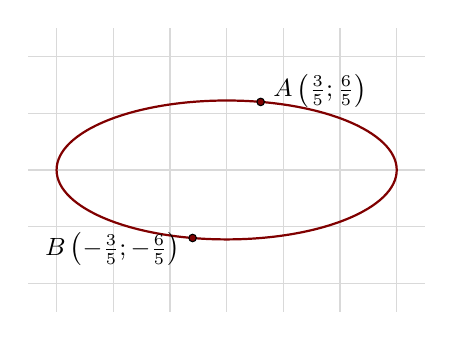
\begin{tikzpicture}[x=8mm, y=8mm,font=\small,scale=.9]
\draw[step=0.8cm,color=gray!30] (-3.5,-2.5) grid (3.5,2.5);
  \tkzInit[xmin=-3.5,xmax=3.5,ymin=-2.5,ymax=2.5]
  \begin{scope}[font=\small]
    \tkzAxeX[below = 3pt]
    \tkzAxeY[left = 1pt]
  \end{scope}
  \tkzFct[domain=-2:2,thick,color=blue]{2*x};

\draw[thick,color=Maroon] (0,0) ellipse (3 and 1.225);
%il punto A
\draw[fill=Maroon] (.6,1.2)circle (1.5pt);
\node[right] at (.65,1.4) {$A \left(\frac{3}{5};\frac{6}{5}\right)$};
%il punto B
\draw[fill=Maroon] (-.6,-1.2)circle (1.5pt);
\node[left] at (-.65,-1.4) {$B \left(-\frac{3}{5};-\frac{6}{5}\right)$};

\end{tikzpicture}

\end{center}
 \end{htmulticols}
\end{esempio}

\begin{esempio}{}{}
Risolvere il seguente sistema: \(\left\{\begin{array}{l}x-y=-2 \\x^2+y-3x-1=0\end{array}\right..\)

Isoliamo la \(y\) dell'equazione di primo grado e sostituiamo nell'equazione di secondo grado 
\[\left\{\begin{array}{l}y=x+2 \\
x^2+\left(x+2\right)-3x-1=0\end{array}\right. 
\Rightarrow\left\{\begin{array}{l}y=x+2 \\
x^2-2x+1=0\end{array}\right.\]

L' \emph{equazione risolvente del sistema}. \(x^2-2x+1=0\) ha il discriminante uguale a zero e due soluzioni reali coincidenti: \(x_1=x_2=1\).

Il sistema ha due soluzioni reali coincidenti, 
\[\left\{\begin{array}{l}y=x+2 \\x^2-2x+1=0\end{array}\right. 
\Rightarrow\left\{\begin{array}{l}x=1 \\
y=1+2=3\end{array}\right.\] 
quindi con soluzione \((1;3)\).
\begin{htmulticols}{2}
Le soluzioni del sistema possono essere interpretate geometricamente come i punti di incontro tra la retta rappresentata dall'equazione \(y=x+2\) e la parabola rappresentata dall'equazione \(y=-x^2+3x+1\). La soluzioni saranno due punti reali coincidenti. Questo punto è detto punto di tangenza tra retta e parabola.
\begin{center}
% (c) 2013 Claudio Carboncini - claudio.carboncini@gmail.com
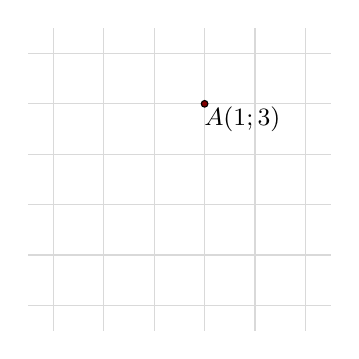
\begin{tikzpicture}[x=8mm, y=8mm,font=\small,scale=.8]
\draw[step=0.8cm,color=gray!30] (-2.5,-1.5) grid (3.5,4.5);
  \tkzInit[xmin=-2.5,xmax=3.5,ymin=-1.5,ymax=4.5]
  \begin{scope}[font=\small]
    \tkzAxeX[below = 3pt]
    \tkzAxeY[left = 1pt]
  \end{scope}
\tkzFct[domain=-.5:3.5,thick,color=Maroon]{-x*x+3*x+1};
\tkzFct[domain=-3.5:6.5,thick,color=blue]{x+2};
%il punto A
\node[right] at (0.8,2.7) {$A (1;3)$};
\draw[fill=Maroon] (1,3)circle (1.5pt);
\end{tikzpicture}

\end{center}
 \end{htmulticols}
\end{esempio}

\begin{esempio}{}{}
Risolvere il seguente sistema: \(\left\{\begin{array}{l}x^2+y^2=4 
\\3x+4y=12\end{array}\right..\)

Isoliamo \(y\) nell'equazione di primo grado e sostituiamola nell'equazione di 
secondo grado 
\[\left\{\begin{array}{l}y=-\frac 3 4x+3 \\
x^2+\left(-\frac 3 4x+3\right)^2-4=0\end{array}\right. 
\Rightarrow\left\{\begin{array}{l}y=-\frac 3 4x+3 \\
x^2+\frac 9{16}x^2-\frac 9 2x+9-4=0\end{array}\right. 
\Rightarrow\left\{\begin{array}{l}y=-\frac 3 4x+3 \\
\frac{25}{16}x^2-\frac{9}{2}x+5=0\end{array}\right..\]

Risolviamo l'equazione di secondo grado in una sola incognita 
\(\frac{25}{16}x^2-\frac 9 2x+5=0\) e verifichiamo che \(\Delta =\frac{81} 
4-\frac{125} 4\) è negativo, quindi l'equazione non ha soluzioni reali e 
\(\IS=\emptyset \). Il sistema non ha soluzioni reali e si dice 
\emph{impossibile}.

\begin{htmulticols}{2}
Le soluzioni del sistema possono essere interpretate geometricamente come 
i punti di incontro tra la retta rappresentata dall'equazione 
\(y=-\frac 3 4x+3\) e la curva rappresentata dall'equazione \(x^2+y^2=4\). 
Nella rappresentazione grafica ottenuta con un software che disegna 
funzioni le figure geometriche ottenute non hanno punti d'incontro.
La curva rappresentata dalla prima equazione è una circonferenza; retta 
e circonferenza non hanno punti di intersezione.
\begin{center}
% (c) 2013 Claudio Carboncini - claudio.carboncini@gmail.com
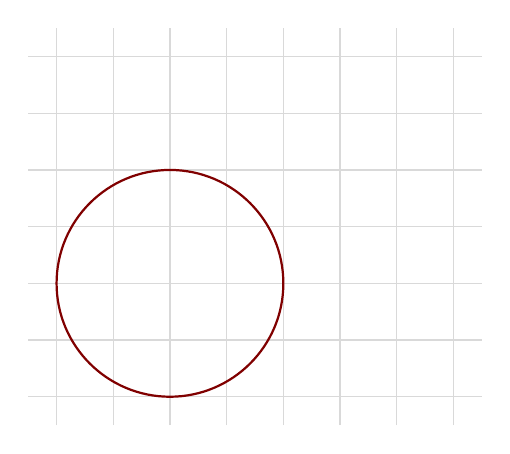
\begin{tikzpicture}[x=8mm, y=8mm,font=\small,scale=.9]
\draw[step=0.8cm,color=gray!30] (-2.5,-2.5) grid (5.5,4.5);
  \tkzInit[xmin=-2.5,xmax=5,ymin=-2.5,ymax=4]
  \begin{scope}[font=\small]
    \tkzAxeX[below = 3pt]
    \tkzAxeY[left = 1pt]
  \end{scope}
\tkzFct[domain=-3:5.5,thick,color=blue]{-0.75*x+3};

\draw[thick,color=Maroon] (0,0) circle (2);
\end{tikzpicture}

\end{center}
 \end{htmulticols}
\end{esempio}

\conclusione
Un sistema di secondo grado, con equazione risolvente di secondo grado,  
rappresenta sempre l'intersezione tra una retta e una curva di secondo 
grado (circonferenza, parabola, ellisse o iperbole). 
Le soluzioni del sistema rappresentano i punti di incontro tra retta e 
curva. 
In base al segno del discriminante dell'equazione risolvente abbiamo:
\begin{itemize*}
\item \(\Delta >0\) le soluzioni del sistema sono le coordinate di due 
punti distinti;
\item \(\Delta =0\) le soluzioni del sistema sono le coordinate di due 
punti coincidenti;
\item \(\Delta <0\) il sistema non ha soluzioni reali. 
Retta e curva non hanno punti in comune.
\end{itemize*}
\begin{center}
% (c) 2013 Claudio Carboncini - claudio.carboncini@gmail.com
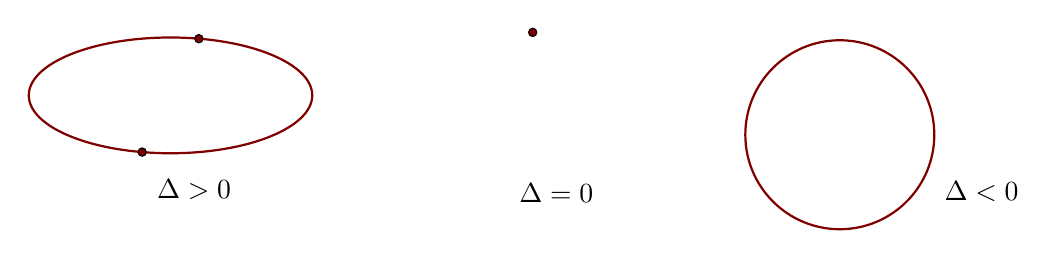
\begin{tikzpicture}[x=6mm, y=6mm]
  \tkzInit[xmin=-3.5,xmax=3.5,ymin=-2.5,ymax=2.5]
  \tkzFct[domain=-2:2,thick,color=blue]{2*x};
\draw[thick,color=Maroon] (0,0) ellipse (3 and 1.225);
\draw[fill=Maroon] (.6,1.2)circle (1.5pt);
\draw[fill=Maroon] (-.6,-1.2)circle (1.5pt);
\node[color =black] at (.5,-2) {$\Delta>0$};

\begin{scope}[xshift=4cm,yshift=-1cm]
\tkzInit[xmin=-2.5,xmax=3.5,ymin=-1.5,ymax=4.5]
\tkzFct[domain=-.5:3.5,thick,color=Maroon]{-x*x+3*x+1};
\tkzFct[domain=-3.5:6.5,thick,color=blue]{x+2};
\draw[fill=Maroon] (1,3)circle (1.5pt);
\node[color =black] at (1.5,-0.4) {$\Delta=0$};
\end{scope}

\begin{scope}[xshift=8.5cm,yshift=-.5cm]
\tkzInit[xmin=-2.5,xmax=5,ymin=-2.5,ymax=4];
\tkzFct[domain=-3:5.5,thick,color=blue]{-0.75*x+3};
\draw[thick,color=Maroon] (0,0) circle (2);
\node[color =black] at (3,-1.2) {$\Delta<0$};
\end{scope}


\end{tikzpicture}

\end{center}

Se l'equazione risolvente risulta essere una equazione di \emph{primo grado} o 
una \emph{uguaglianza} vera o falsa, allora:
\begin{itemize*}
\item se si ottiene una uguaglianza vera, il sistema è indeterminato;
\item se si ottiene una uguaglianza falsa il sistema è impossibile;
\item se l'equazione risolvente è di primo grado determinata, da essa si ricava 
il valore dell'incognita e si sostituisce tale valore nell'altra equazione. Il 
sistema ha una sola soluzione (in questo caso non si parla di due soluzioni 
coincidenti, come nel caso precedente di \(\Delta =0\)).
\end{itemize*}

\begin{esempio}{}{}
Risolvere il sistema 
\(\left\{\begin{array}{l}x^2-y^2=0\\x+y=0\end{array}\right.\).

Isoliamo la \(y\) dell'equazione di primo grado e sostituiamo nell'equazione di 
secondo grado. 
\[\left\{\begin{array}{l}y=-x \\
x^2-(-x)^2=0\end{array}\right.\ 
\Rightarrow\left\{\begin{array}{l}y=-x \\
x^2-x^2=0\end{array}\right. 
\Rightarrow\left\{\begin{array}{l}y=-x\\
0=0\end{array}\right..\]

L' \emph{equazione risolvente del sistema} in questo caso è una \emph{identità} 
(uguaglianza vera) e tutte le coppie formate da numeri opposti (la prima 
equazione ci vincola ad avere \(y=-x\) ) sono soluzioni del sistema: \(\forall 
k\in \mathbb{R}\Rightarrow {I.S.}=(k;-k)\). Il sistema ha infinite coppie di 
numeri reali che lo soddisfano e si dice \emph{indeterminato}.
\begin{htmulticols}{2}
La figura è quella che otteniamo se inseriamo le due equazioni in un software 
che disegna funzioni. La curva di secondo grado è formata dalle due rette 
\(x+y=0\) e \(x-y=0\) e la seconda equazione rappresenta la retta a che si 
sovrappone alla precedente.
\begin{center}
% (c) 2013 Claudio Carboncini - claudio.carboncini@gmail.com

\begin{tikzpicture}[x=6mm, y=6mm,font=\small,scale=.7]
\draw[step=0.6cm,color=gray!30] (-4.5,-4.5) grid (4.5,4.5);
  \tkzInit[xmin=-4.5,xmax=4.5,ymin=-4.5,ymax=4.5]
  \begin{scope}[font=\small]
    \tkzAxeX[below = 3pt]
    \tkzAxeY[left = 1pt]
  \end{scope}
    \tkzFct[domain=-4.5:4.5,thick,color=blue]{x};
    \tkzFct[domain=-4.5:4.5,very thick,color=Maroon]{-x};
\end{tikzpicture}

\end{center}
\end{htmulticols}
\end{esempio}

\begin{esempio}{}{}
Risolvere il sistema \(\left\{\begin{array}{l}\frac 3 
2x+y=0\\x^2-y^2=4\end{array}\right..\)

Isoliamo la \(y\) dell'equazione di primo grado e sostituiamo nell'equazione di 
secondo grado 
\[\left\{\begin{array}{l}y=-\frac 3 2x \\
x^2-\left(-\frac 3 2x\right)^2=4\end{array}\right.
\Rightarrow \left\{\begin{array}{l}y=-\frac 3 2x \\
x^2-\frac 9 4x^2=4\end{array}\right.
\Rightarrow \left\{\begin{array}{l}y=-\frac 3 2x\\
-\frac 5 4x^2=4\end{array}\right..\]

L' equazione risolvente del sistema \(-\frac 5 4x^2=4\) non ha soluzioni, quindi 
il sistema è \emph{impossibile}.
\begin{htmulticols}{2}
La figura è quella che otteniamo se inseriamo le due equazioni in un software 
che disegna le funzioni. L'equazione di secondo grado rappresenta una curva 
detta iperbole e la seconda equazione rappresenta la retta; vediamo che curva e 
retta non hanno punti di intersezione.
\begin{center}
% (c) 2013 Claudio Carboncini - claudio.carboncini@gmail.com
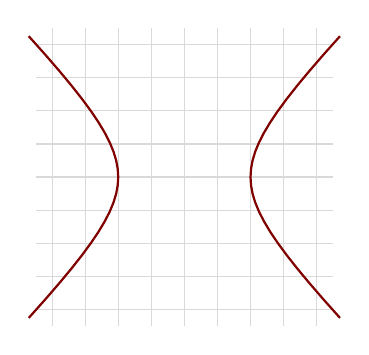
\begin{tikzpicture}[x=6mm, y=6mm,font=\small,scale=.7]
\draw[step=0.6cm,color=gray!30] (-4.5,-4.5) grid (4.5,4.5);
  \tkzInit[xmin=-4.5,xmax=4.5,ymin=-4.5,ymax=4.5]
  \begin{scope}[font=\small]
    \tkzAxeX[below = 3pt]
    \tkzAxeY[left = 1pt]
  \end{scope}
   \pgfmathsetmacro{\e}{1.41421}   % eccentricity
    \pgfmathsetmacro{\a}{2}
    \pgfmathsetmacro{\b}{(\a*sqrt((\e)^2-1)} 
    \draw[thick,color=Maroon] plot[domain=-1.5:1.5] ({\a*cosh(\x)},{\b*sinh(\x)});
    \draw[thick,color=Maroon] plot[domain=-1.5:1.5] ({-\a*cosh(\x)},{\b*sinh(\x)});
    \tkzFct[domain=-4:4,thick,color=blue]{-1.5*x};
\end{tikzpicture}

\end{center}
\end{htmulticols}
\end{esempio}

\begin{esempio}{}{}
Risolvere il sistema 
\(\left\{\begin{array}{l}x^2-y^2=4\\-x+y=-1\end{array}\right.\).

Isoliamo la \(y\) dell'equazione di primo grado e sostituiamo nell'equazione di 
secondo grado 
\[\left\{\begin{array}{l}y=x-1 \\
x^2-(x-1)^2-4=0\end{array}\right.
\Rightarrow \left\{\begin{array}{l}y=x-1 \\
x^2-x^2+2x-1-4=0\end{array}\right.
\Rightarrow \left\{\begin{array}{l}y=x-1\\2x=5\end{array}\right..\]

L' \emph{equazione risolvente del sistema} in questo caso è l'equazione di primo 
grado \(2x-5=0\), la cui soluzione è \(x=\frac 5 2\). Si sostituisce il valore 
trovato nell'altra equazione e troviamo la soluzione del sistema che in questo 
caso è unica: 
\[\left\{\begin{array}{l}y=x-1 \\2x=5\end{array}\right. 
\Rightarrow\left\{\begin{array}{l}x=\frac 5 2 \\
y=\frac 5 2-1=\frac 3 2\end{array}\right.\] 
quindi con soluzione \[\left(\frac 5 2;\frac 3 2\right).\]

\begin{htmulticols}{2}
La figura è quella che otteniamo se inseriamo le due equazioni in un applicativo 
che disegna funzioni. L'equazione di secondo grado rappresenta una curva detta 
iperbole e la seconda equazione rappresenta una retta; vediamo che curva e retta 
hanno un solo punto di intersezione.
\begin{center}
% (c) 2013 Claudio Carboncini - claudio.carboncini@gmail.com
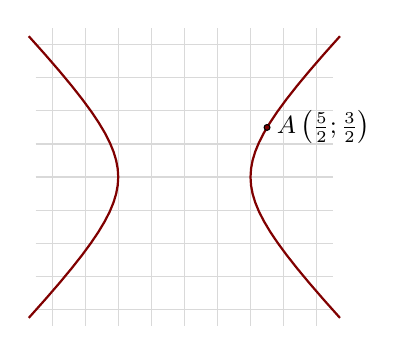
\begin{tikzpicture}[x=6mm, y=6mm,font=\small,scale=.7]
\draw[step=0.6cm,color=gray!30] (-4.5,-4.5) grid (4.5,4.5);
  \tkzInit[xmin=-4.5,xmax=4.5,ymin=-4.5,ymax=4.5]
  \begin{scope}[font=\small]
    \tkzAxeX[below = 3pt]
    \tkzAxeY[left = 1pt]
  \end{scope}
   \pgfmathsetmacro{\e}{1.41421}   % eccentricity
    \pgfmathsetmacro{\a}{2}
    \pgfmathsetmacro{\b}{(\a*sqrt((\e)^2-1)} 
    \draw[thick,color=Maroon] plot[domain=-1.5:1.5] ({\a*cosh(\x)},{\b*sinh(\x)});
    \draw[thick,color=Maroon] plot[domain=-1.5:1.5] ({-\a*cosh(\x)},{\b*sinh(\x)});
    \tkzFct[domain=-4:5,thick,color=blue]{x-1};
    \node[right] at (2.5,1.5) {$A \left(\frac 5 2;\frac 3 2\right)$};
    \draw[fill=Maroon] (2.5,1.5)circle (1.5pt);
\end{tikzpicture}

\end{center}
\end{htmulticols}
\end{esempio}

% \ovalbox{\risolvii \ref{ese:6.1}, \ref{ese:6.2}, \ref{ese:6.3}, 
% \ref{ese:6.4}, \ref{ese:6.5}, \ref{ese:6.6}, \ref{ese:6.7}.}

\subsection{Sistemi di secondo grado letterali}

\begin{esempio}{}{}
Discutere e risolvere il seguente sistema: 
\(\left\{\begin{array}{l}y-kx=-2\\y-x^2=2\end{array}\right.\).

Si risolve come nel caso degli analoghi sistemi numerici. Bisognerà, 
nell'equazione risolvente, discutere per quali valore del parametro si 
otterranno soluzioni reali. Ricaviamo la y dalla prima equazione e sostituiamo 
nella seconda equazione:
\[ \left\{\begin{array}{l}y=kx-2\\kx-2-x^2=2\end{array}\right.\ 
\Rightarrow\left\{\begin{array}{l}y=kx-2\\-x^2+kx-4=0\end{array}\right.\ 
\Rightarrow\left\{\begin{array}{l}y=kx-2\\x^2-kx+4=0\end{array}\right.. \]

Discutiamo e risolviamo l'equazione di secondo grado 
\[ \Delta =k^2-16 \Rightarrow
\begin{array}{l}\Delta >0\Rightarrow k<-4\vee k>4\Rightarrow 
x_1=\frac{k-\sqrt{k^2-16}} 2\vee x_2=\frac{k+\sqrt{k^2-16}} 2\\
\Delta =0\Rightarrow k=-4\vee k=4\Rightarrow x_1=x_2=\frac k 2 \\
\Delta <0\Rightarrow -4<k<4\Rightarrow \IS=\emptyset \end{array}. \]

Ricaviamo i valori della x che sostituiamo nella prima equazione: \[ 
\left\{\begin{array}{l}y-kx=-2\\y-x^2=2\end{array}\right.\text{ se }k\le -4\vee 
k\ge 4\Rightarrow \left\{\begin{array}{l}x_1=\frac{k-\sqrt{k^2-16}} 2 
\\y_1=\frac{k^2-4-k\sqrt{k^2-16}} 2\end{array}\right.\vee 
\left\{\begin{array}{l}x_2=\frac{k+\sqrt{k^2-16}} 2 
\\y_2=\frac{k^2-4+k\sqrt{k^2-16}} 2\end{array}\right.. \]
\end{esempio}

% \ovalbox{\risolvii \ref{ese:6.8}, \ref{ese:6.9}.}

\subsection{Sistemi frazionari}
Si dice frazionario un sistema in cui almeno una delle equazioni che lo 
compongono è frazionaria; per questo motivo occorre procedere alla definizione 
del Dominio in cui si ricercano le soluzioni del sistema.

\begin{esempio}{}{}
Risolvere il seguente sistema \(\left\{\begin{array}{l}2x-y=2 \\\frac 
x{y+2}=\frac x{2y+5}\end{array}\right.\).

Determiniamo le condizioni di esistenza di \( \frac x{y+2}=\frac x{2y+5} \):\; 
\(\CE y\neq -2\wedge y\neq -\frac 5 2\).

Trasformiamo l'equazione frazionaria nella sua forma canonica di equazione 
intera:
\begin{align*}
 &\frac x{y+2}=\frac x{2y+5}\\
\Rightarrow & x\cdot (2y+5)-x\cdot (y+2)=0\\
\Rightarrow & 2{xy}+5x-{xy}-2x=0\\
\Rightarrow & xy+3x=0.
\end{align*}

Il sistema diventa: 
\[\left\{\begin{array}{l}y=2x-2\\
xy+3x=0\end{array}\right.
\Rightarrow \left\{\begin{array}{l}y=2x-2\\
x(2x-2)+3x=0\end{array}\right.
\Rightarrow \left\{\begin{array}{l}y=2x-2\\
2x^2+x=0\end{array}\right..\]

 \(2x^2+x=0\) è l'equazione risolvente; ha soluzioni \(x_1=0\vee x_2=-\frac 1 
2\).

Sostituiamo le soluzioni trovate nell'equazione di primo grado e otteniamo le 
soluzioni del sistema: 
\[\left\{\begin{array}{l}x_1=0 \\
y_1=-2\end{array}\right.\vee 
\left\{\begin{array}{l}x_2=-\frac 1 2\\
y_2=-3\end{array}\right. 
\Rightarrow\left(0;-2\right)\vee \left(-\frac 1 2;-3\right).\]

La soluzione \((0;-2)\) non soddisfa le \(\CE\) Il sistema ha soluzione 
\(\left(-\frac 1 2;-3\right)\).
\end{esempio}

% \ovalbox{\risolvii \ref{ese:6.10}, \ref{ese:6.11}}

\subsubsection{Sistemi di secondo grado in tre incognite}
Quanto detto si può estendere ai sistemi di secondo grado di tre o più equazioni 
con altrettante incognite. Per risolvere uno di tali sistemi si cercherà, 
operando successive sostituzioni a partire dalle equazioni di primo grado, di 
ottenere un'equazione di secondo grado in una sola incognita (equazione 
risolvente del sistema).

A partire dalle eventuali soluzioni di tale equazione, si determineranno poi le 
soluzioni del sistema.

\newpage

\begin{esempio}{}{}
Risolvere il sistema 
\(\left\{\begin{array}{l}2x+y-z=0\\3x+4y-2z=1\\xy-y^2+z-5y=0\end{array}\right.\)
.

Isoliamo \( z \) dalla prima equazione, che è di primo grado, e sostituiamo 
nelle altre equazioni: 
\[ \left\{\begin{array}{l}z=2x+y\\
3x+4y-2(2x+y)=1\\
{xy}-y^2+(2x+y)-5y=0\end{array}\right. 
\Rightarrow\left\{\begin{array}{l}z=2x+y\\
3x+4y-4x-2y=1\\
xy-y^2+2x-4y=0\end{array}\right. \Rightarrow\left\{\begin{array}{l}z=2x+y\\
-x+2y-1=0\\
xy-y^2+2x-4y=0\end{array}\right..\]

Ricaviamo \( x \) dalla seconda equazione e la sostituiamo nelle altre 
equazioni: 
\[ \left\{\begin{array}{l}z=2(2y-1)+y\\
x=2y-1\\
2y^2-y-y^2+4y-2-4y=0\end{array}\right. 
\Rightarrow\left\{\begin{array}{l}z=5y-2\\
x=2y-1\\
y^2-y-2=0\end{array}\right..\]

L'equazione \(y^2-y-2=0\) è l'equazione risolvente del sistema, le sue soluzioni 
sono \(y_1=2\vee y_2=-1\).

Sostituiamo i valori trovati per la \( y \) nelle altre equazioni per trovare i 
valori corrispondenti della \( x \) e della \( z \): \[ 
\left\{\begin{array}{l}z=5(2)-2=8 \\x=2(2)-1=3 \\y=2 \end{array}\right.\vee 
\left\{\begin{array}{l}z=5(-1)-2=-7 \\x=2(-1)-1=-3 \\y=-1 
\end{array}\right.\Rightarrow (3;2;8)\vee (-3;-1;-7). \]
\end{esempio}

% \ovalbox{\risolvii \ref{ese:6.12}, \ref{ese:6.13}}

\section{Sistemi simmetrici}
Un sistema di due equazioni in due incognite si dice \emph{simmetrico} se non 
cambia scambiando le incognite.

Per esempio, nel sistema 
\[\left\{\begin{array}{l}{x+y=1}\\{x^2+y^2+3{xy}+5=0}\end{array}\right.\] se 
scambiamo la \(x\) con la \(y\) otteniamo 
\[\left\{\begin{array}{l}{y+x=1}\\{y^2+x^2+3{yx}+5=0}\end{array}\right.\] che è 
identico al precedente.

Risolviamo il sistema, le soluzioni sono 
\[\left\{\begin{array}{l}{x_1=-2}\\{y_1=3}\end{array}\right.\vee 
\left\{\begin{array}{l}{x_2=3}\\{y_2=-2}\end{array}\right.\] 
e come si può notare \(x\) e \(y\) vengono scambiate anche nella soluzione.

In generale se il sistema è simmetrico trovata una coppia soluzione \((a;b)\) 
l'altra è \((b;a)\).

\subsection{Sistemi simmetrici di secondo grado}
Il sistema simmetrico fondamentale è del tipo 
\(\left\{\begin{array}{l}{x+y=s}\\{xy=p}\end{array}\right.\) esso risolve il 
problema di trovare due numeri, nota la loro somma e il loro prodotto.

Ricordiamo che nell'equazione di secondo grado \(x^2+bx+c=0\), la somma delle 
radici è \(-b\), mentre il prodotto è \(c\). Pertanto, basta risolvere la 
seguente equazione, \emph{detta equazione risolvente: } \(t^2-st+p=0\) con 
\(s=-b\) e \(p=c\).

In base al segno del discriminante abbiamo:
\begin{itemize*}
\item \(\Delta >0\) l'equazione risolvente ha due soluzioni distinte \( t_1 \) e 
\( t_2 \), le soluzioni del sistema sono: 
\(\left\{\begin{array}{l}{x_1=t_1}\\{y_1=t_2}\end{array}\right.\vee 
\left\{\begin{array}{l}{x_2=t_2}\\{y_2=t_1}\end{array}\right.\)
\item \(\Delta =0\) l'equazione risolvente ha radici coincidenti \(t_1=t_2\), le 
soluzioni del sistema sono: 
\(\left\{\begin{array}{l}{x_1=t_1}\\{y_1=t_1}\end{array}\right.\vee 
\left\{\begin{array}{l}{x_2=t_1}\\{y_2=t_1}\end{array}\right.\)
\item \(\Delta <0\) l'equazione non ammette soluzioni reali. Il sistema è 
impossibile.
\end{itemize*}

\begin{esempio}{}{}
Risolvere il seguente sistema 
\(\left\{\begin{array}{l}{x+y=5}\\{xy=4}\end{array}\right.\).
\begin{htmulticols}{2}
L'equazione risolvente è \(t^2-5t+4=0\) le cui soluzioni sono: \(t_1=1\vee 
t_2=4\).

Le soluzioni del sistema sono le seguenti: \[ 
\left\{\begin{array}{l}{x_1=1}\\{y_1=4}\end{array}\right.\vee 
\left\{\begin{array}{l}{x_2=4}\\{y_2=1}\end{array}\right.. \]

Possiamo interpretare i risultati ottenuti nel piano cartesiano: la retta di 
equazione \(x+y=5\) interseca l'iperbole equilatera \({xy}=4\) nei due punti 
\(A(1;4)\) e \(B(4;1)\).
\begin{center}
% (c) 2013 Claudio Carboncini - claudio.carboncini@gmail.com
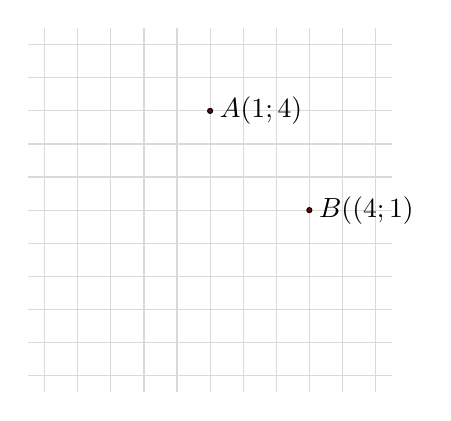
\begin{tikzpicture}[x=7mm, y=7mm, scale=.6]
\draw[step=0.7cm,color=gray!30] (-4.5,-4.5) grid (6.5,6.5);
  \tkzInit[xmin=-4,xmax=6,ymin=-4,ymax=6]
  \begin{scope}[font=\small]
    \tkzAxeX[below = 3pt]
    \tkzAxeY[left = 1pt]
  \end{scope}
  \tkzFct[domain=-5.5:0,thick,color=Maroon]{4/x}
  \tkzFct[domain=-0:5.5,thick,color=Maroon]{4/x}
\tkzFct[domain=-2:6,thick,color=blue]{-x+5};
 \draw[fill=Maroon] (1,4)circle (1.5pt);
\node[right] at (1,4) {$A (1;4)$};
\draw[fill=Maroon] (4,1)circle (1.5pt);
\node[right] at (4,1) {$B ((4;1)$};

\end{tikzpicture}

\end{center}
\end{htmulticols}
\end{esempio}

\begin{esempio}{}{}
Risolvere il seguente sistema 
\(\left\{\begin{array}{l}{x+y=1}\\{xy=4}\end{array}\right.\).
\begin{htmulticols}{2}
L'equazione risolvente è \[ t^2-t+4=0 \] con il discriminante negativo e dunque 
senza soluzioni reali. Il sistema è impossibile.

Possiamo interpretare i risultati ottenuti nel piano cartesiano: la retta di 
equazione \(x+y=1\) non interseca l'iperbole equilatera \({xy}=4\).
\begin{center}
% (c) 2013 Claudio Carboncini - claudio.carboncini@gmail.com

\begin{tikzpicture}[x=7mm, y=7mm, scale=.6]
\draw[step=0.7cm,color=gray!30] (-4.5,-4.5) grid (4.5,4.5);
  \tkzInit[xmin=-4.5,xmax=4.5,ymin=-4.5,ymax=4.5]
  \begin{scope}[font=\small]
    \tkzAxeX[below = 3pt]
    \tkzAxeY[left = 1pt]
  \end{scope}
  \tkzFct[domain=-4.5:0,thick,color=Maroon]{1/x}
  \tkzFct[domain=-0:4.5,thick,color=Maroon]{1/x}
\tkzFct[domain=-3:4,thick,color=blue]{-x+1};
\end{tikzpicture}

\end{center}
\end{htmulticols}
\end{esempio}
\newpage
\begin{esempio}{}{}
Risolvere il seguente sistema \(\left\{\begin{array}{l}{x+y=2}\\{xy=1}\end{array}\right.\).
\begin{htmulticols}{2}
L'equazione risolvente è \(t^2-2t+1=0\) le cui soluzioni sono: \(t_1=t_2=1\).

Il sistema ha due soluzioni coincidenti: \[ \left\{\begin{array}{l}{x_1=1}\\{y_1=1}\end{array}\right.\vee \left\{\begin{array}{l}{x_2=1}\\{y_2=1}\end{array}\right.. \]

Possiamo interpretare i risultati ottenuti nel piano cartesiano: la retta di equazione \(x+y=2\) è tangente all'iperbole equilatera \(xy=1\) nel punto \((1;1)\).
\begin{center}
% (c) 2013 Claudio Carboncini - claudio.carboncini@gmail.com
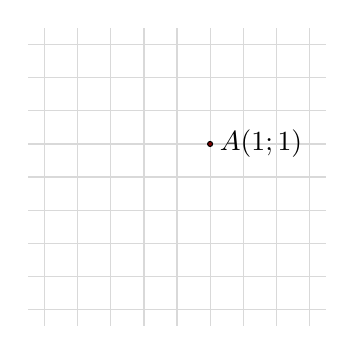
\begin{tikzpicture}[x=7mm, y=7mm, scale=.6]
\draw[step=0.7cm,color=gray!30] (-4.5,-4.5) grid (4.5,4.5);
  \tkzInit[xmin=-4.5,xmax=4.5,ymin=-4.5,ymax=4.5]
  \begin{scope}[font=\small]
    \tkzAxeX[below = 3pt]
    \tkzAxeY[left = 1pt]
  \end{scope}
  \tkzFct[domain=-4.5:0,thick,color=Maroon]{1/x}
  \tkzFct[domain=-0:4.5,thick,color=Maroon]{1/x}
\tkzFct[domain=-3:4,thick,color=blue]{-x+2};
\draw[fill=Maroon] (1,1)circle (1.5pt);
 \node[right] at (1,1) {$A (1;1)$};
\end{tikzpicture}

\end{center}
\end{htmulticols}
\end{esempio}

% \ovalbox{\risolvii \ref{ese:6.14}, \ref{ese:6.15}, \ref{ese:6.16}, 
% \ref{ese:6.17}, \ref{ese:6.18}, \ref{ese:6.19}}

\subsection{Sistemi simmetrici riconducibili al sistema simmetrico fondamentale}
In questa categoria rientrano i sistemi simmetrici che, mediante artifici, 
possono essere trasformati in sistemi simmetrici del tipo precedente.

\begin{esempio}{}{}
Risolvere il sistema 
\(\left\{\begin{array}{l}{x+y=a}\\{x^2+y^2+{bx}+{by}=c}\end{array}\right.\).

È possibile trasformare il sistema in un sistema simmetrico fondamentale.

Ricordando l'identità \(x^2+y^2=(x+y)^2-2{xy}\), il sistema può essere riscritto 
così: 
\[ \left\{\begin{array}{l}{x+y=a}\\
{(x+y)^2-2{xy}+b(x+y)=c}\end{array}\right.
\Rightarrow \left\{\begin{array}{l}{x+y=a}\\
{a^2-2{xy}+{ba}=c}\end{array}\right.
\Rightarrow \left\{\begin{array}{l}{x+y=a}\\
{{xy}=\frac{a^2+{ab}-c} 2}\end{array}\right..\]

Posto \(a=s\) e \(p=\frac{a^2+{ab}-c} 2\) il sistema diventa 
\[\left\{\begin{array}{l}{x+y=s}\\{{xy}=p}\end{array}\right..\]
\end{esempio}

\begin{esempio}{}{}
Risolvere il sistema 
\(\left\{\begin{array}{l}{x+y=7}\\{x^2+y^2=25}\end{array}\right.\)

Ricordando l'identità \(x^2+y^2=(x+y)^2-2{xy}\), il sistema può essere riscritto 
così: 
\[\left\{\begin{array}{l}{x+y=7}\\
{(x+y)^2-2{xy}=25}\end{array}\right.
\Rightarrow \left\{\begin{array}{l}{x+y=7}\\
{(7)^2-2{xy}=25}\end{array}\right.
\Rightarrow \left\{\begin{array}{l}{x+y=7}\\
{-2{xy}=25-49}\end{array}\right.\Rightarrow 
\left\{\begin{array}{l}{x+y=7}\\{{xy}=12}\end{array}\right..\]

L'equazione risolvente è \(t^2-7t+12=0\) le cui soluzioni sono \(t_1=3\vee 
t_2=4\).

Le soluzioni del sistema sono: 
\[\left\{\begin{array}{l}{x_1=3}\\
{y_1=4}\end{array}\right.\vee \left\{\begin{array}{l}{x_2=4}\\
{y_2=3}\end{array}\right..\]
\end{esempio}

\begin{esempio}{}{}
Risolvere il sistema 
\(\left\{\begin{array}{l}{-3x-3y=-5}\\{2x^2+2y^2=10}\end{array}\right.\)

Dividendo per \(-3\) la prima equazione, per \(2\) la seconda e ricordando 
l'identità 
\[x^2+y^2=(x+y)^2-2{xy}\] 
si ha: 
\[ \left\{\begin{array}{l}{x+y=\frac 5 3}\\
{x^2+y^2=5}\end{array}\right.
\Rightarrow \left\{\begin{array}{l}{x+y=\frac 5 3}\\
{(x+y)^2-2{xy}=5}\end{array}\right.
\Rightarrow \left\{\begin{array}{l}{x+y=\frac 5 3}\\
{\left(\frac 5 3\right)^2-2{xy}=5}\end{array}\right.
\Rightarrow \left\{\begin{array}{l}{x+y=\frac 5 3}\\
{{xy}=-\frac{10} 9}\end{array}\right..\]

L'equazione risolvente è \(t^2-\frac 5 3t-\frac{10} 9=0\) le cui soluzioni sono: 
\(t_1=\frac{5-\sqrt{65}} 6\vee t_2=\frac{5+\sqrt{65}} 6\).

Le soluzioni del sistema sono le seguenti: 
\[\left\{\begin{array}{l}{x_1=\frac{5-\sqrt{65}} 6}\\{y_1=\frac{5+\sqrt{65}} 
6}\end{array}\right.\vee \left\{\begin{array}{l}{x_2=\frac{5+\sqrt{65}} 
6}\\{y_2=\frac{5-\sqrt{65}} 6}\end{array}\right..\]
\end{esempio}

% \ovalbox{\risolvii \ref{ese:6.20}, \ref{ese:6.21}, \ref{ese:6.22}, 
% \ref{ese:6.23}, \ref{ese:6.24}}

\subsection{Sistemi non simmetrici riconducibili a sistemi simmetrici}
Rientrano in questa classe i sistemi che, pur non essendo simmetrici, possono 
essere trasformati, mediante opportune sostituzioni, in sistemi simmetrici. 
Naturalmente questi sistemi si possono risolvere anche con la procedura solita 
di sostituzione per i sistemi di secondo grado.

\begin{esempio}{}{}
Risolvere il sistema 
\(\left\{\begin{array}{l}{x-y=8}\\{{xy}=-15}\end{array}\right.\).

Mediante la sostituzione \(y'=-y\) otteniamo 
\(\left\{\begin{array}{l}{x+y'=8}\\{xy'=15}\end{array}\right.\) che è un sistema 
simmetrico fondamentale.

L'equazione risolvente è \(t^2-8t+15=0\) le cui soluzioni sono \(t_1=3\vee 
t_2=5\), pertanto il sistema ha le soluzioni 
\[\left\{\begin{array}{l}{x_1=3}\\
{{y_1}'=5}\end{array}\right.\vee 
\left\{\begin{array}{l}{x_2=5}\\
{{y_2}'=3}\end{array}\right..\] 
Dall'uguaglianza \(y'=-y\Rightarrow y=-y'\) otteniamo le soluzioni del sistema 
dato 
\[\left\{\begin{array}{l}{x_1=3}\\
{y_1=-5}\end{array}\right.\vee 
\left\{\begin{array}{l}{x_2=5}\\
{y_2=-3}\end{array}\right..\]
\end{esempio}

\begin{esempio}{}{}
Risolvere il sistema 
\(\left\{\begin{array}{l}{2x-3y=8}\\{{xy}=2}\end{array}\right.\).

Mediante la sostituzione \(x'=2x\) e \(y'=-3y\) da cui \(x=\frac{x'} 2\) e 
\(y=-\frac{y'} 3\) otteniamo 
\[\left\{\begin{array}{l}{x'+y'=8}\\
{\frac{x'} 2\cdot \left(-\frac{y'} 3\right)=2}\end{array}\right.
\Rightarrow\left\{\begin{array}{l}{x'+y'=8}\\
{x'y'=-12}\end{array}\right.\] che è un sistema simmetrico fondamentale.

Risolviamo il sistema simmetrico 
\(\left\{\begin{array}{l}{x'+y'=8}\\{x'y'=-12}\end{array}\right.\) con la 
procedura nota. L'equazione risolvente è \(t^2-8t-12=0\) le cui soluzioni sono 
\(t_{1,2}=4\pm 2\sqrt 3\) pertanto il sistema ha le soluzioni: 
\[\left\{\begin{array}{l}{x_1'=4-2\sqrt 7}\\
{y_1'=4+2\sqrt 7}\end{array}\right.\vee 
\left\{\begin{array}{l}{x_2'=4+2\sqrt 7}\\
{y_2'=4-2\sqrt 7}\end{array}\right..\] 
Dalle sostituzioni \(x=\frac{x'} 2\) e \(y=-\frac{y'} 3\) otteniamo le soluzioni 
del sistema iniziale 
\[\left\{\begin{array}{l}{x_1=\frac{4-2\sqrt 7} 2=2-\sqrt 7}\\
{y_1=\frac{-4-2\sqrt 7} 3}\end{array}\right.\vee 
\left\{\begin{array}{l}{x_2=\frac{4+2\sqrt 7} 2=2+\sqrt 7}\\
{y_2=\frac{-4+2\sqrt 7} 3}\end{array}\right..\]
\paragraph{Procedura di sostituzione}
Ricaviamo una delle due incognite dall'equazione di primo grado e sostituiamola 
nell'altra equazione \[ \left\{\begin{array}{l}{2x-3y=8} 
\\{{xy}=2}\end{array}\right.\Rightarrow\left\{\begin{array}{l}{y=\frac{2x-8} 
3}\\{{xy}=2}\end{array}\right.\Rightarrow \left\{\begin{array}{l}{y=\frac{2x-8} 
3}\\{x\left(\frac{2x-8} 3\right)=2}\end{array}\right.\Rightarrow 
\left\{\begin{array}{l}{y=\frac{2x-8} 3}\\{2x^2-8x-6=0}\end{array}\right.. \]

Risolviamo l'equazione \(2x^2-8x-6=0\) avente come soluzioni \(x_1=2-\sqrt 7\vee 
x_2=2+\sqrt 7\). Applicando la formula ridotta otteniamo: \(x_1=2-\sqrt 7\vee 
x_2=2+\sqrt 7\).
Sostituiamo i valori trovati e ricaviamo i valori della \(y\): \[ 
\left\{\begin{array}{l}{x_1=2-\sqrt 7}\\{y_1=\frac{-4-2\sqrt 7} 
3}\end{array}\right.\vee \left\{\begin{array}{l}{x_2=2+\sqrt 
7}\\{y_2=\frac{-4+2\sqrt 7} 3}\end{array}\right.. \]
\end{esempio}

% \ovalbox{\risolvi \ref{ese:6.25}}

\subsection{Sistemi simmetrici di grado superiore al secondo}
Introduciamo le seguenti trasformazioni dette formule di Waring, dal nome del 
matematico che le ha formulate per primo. Con tali formule, si possono 
trasformare le potenze di un binomio in relazioni tra somme e prodotti delle due 
variabili che lo compongono. Indicate come \(s\) somma delle variabili e \(p\) 
il loro prodotto queste sono le prime formule fino alla potenza quinta.
\begin{itemize*}
\item \( a^2+b^2=(a+b)^2-2{ab}=s^2-2p \)
\item \( a^3+b^3=(a+b)^3-3a^2b-3ab^2=(a+b)^3-3{ab}(a+b)=s^3-3{ps} \)
\item \( a^4+b^4=s^4-4{ps}^2+2p^2 \)
\item \( a^5+b^5=s^5-5{ps}^3+5p^2s \).
\end{itemize*}

\begin{esempio}{}{}
Risolvere il sistema 
\(\left\{\begin{array}{l}{x+y=1}\\{x^3+y^3-2{xy}=3}\end{array}\right.\).

Applicando l'identità \(x^3+y^3=(x+y)^3-3{xy}(x+y)\), il sistema può essere 
riscritto così: \[ 
\left\{\begin{array}{l}{x+y=1}\\{(x+y)^3-3{xy}(x+y)-2{xy}=3}\end{array}\right.\
Rightarrow 
\left\{\begin{array}{l}{x+y=1}\\{1-5{xy}=3}\end{array}\right.\Rightarrow 
\left\{\begin{array}{l}{x+y=1}\\{{xy}=-\frac 2 5}\end{array}\right..\]

Da cui l'equazione risolvente \(t^2-t-\frac 2 5=0\Rightarrow 5t^2-5t-2=0\) con 
\(t_1=\frac{5-\sqrt{65}}{10}\) e \(t_2=\frac{5+\sqrt{65}}{10}\).
Le soluzioni del sistema sono: 
\(\left(\frac{5-\sqrt{65}}{10};\frac{5+\sqrt{65}}{10}\right),\left(\frac{5+\sqrt
{65}}{10};\frac{5-\sqrt{65}}{10}\right)\).
\end{esempio}

\begin{esempio}{}{}
Risolvere il sistema \(\left\{\begin{array}{l}{x+y=-1}\\{x^4+y^4=\frac 7 
2}\end{array}\right.\).

Ricordando l'identità \(x^4+y^4=(x+y)^4-4{xy}(x+y)^2+2x^2y^2\), il sistema può 
essere riscritto così: 
\[\left\{\begin{array}{l}{x+y=-1}\\{(x+y)^4-4{xy}(x+y)^2+2x^2y^2=\frac 7 
2}\end{array}\right. \Rightarrow 
\left\{\begin{array}{l}{x+y=-1}\\{2x^2y^2-4{xy}-\frac 5 
2=0}\end{array}\right..\]

Introduciamo l'incognita ausiliaria \(u=xy\). L'equazione \(2x^2y^2-4{xy}-\frac 
5 2=0\) diventa \(2u^2-4u-\frac 5 2=0\) che ha come soluzioni \(u_1=-\frac 1 
2\vee u_2=\frac 5 2\Rightarrow {xy}=-\frac 1 2\vee {xy}=\frac 5 2\).

Il sistema assegnato è equivalente a due insiemi 
\[\left\{\begin{array}{l}{x+y=-1}\\{{xy}=-\frac 1 2}\end{array}\right.\vee 
\left\{\begin{array}{l}{x+y=-1}\\{{xy}=\frac 5 2}\end{array}\right.\] 
e dunque il suo insieme soluzione \(S\) si ottiene dall'unione dell'insieme 
soluzione dei due 
sistemi~\(S=S_1\cup S_2\).

Il primo sistema 
\[\left\{\begin{array}{l}{x+y=-1}\\{{xy}=-\frac 1 2}\end{array}\right.\] 
ha equazione risolvente \(t^2+t-\frac 1 2=0\) con 
\[t_1=\frac{-1-\sqrt 3} 2\text{ e }t_2=\frac{-1+\sqrt 3} 2.\] 
Il sistema ha soluzioni 
\[\left(\frac{-1-\sqrt 3} 2;\frac{-1+\sqrt 3} 2\right),\left(\frac{-1+\sqrt 3} 
2;\frac{-1-\sqrt 3} 2\right)\] e quindi \[S_1=\left\{\left(\frac{-1-\sqrt 3} 
2;\frac{-1+\sqrt 3} 2\right),\left(\frac{-1+\sqrt 3} 2;\frac{-1-\sqrt 3} 
2\right)\right\}.\]

Il secondo sistema \(\left\{\begin{array}{l}{x+y=-1}\\{{xy}=\frac 5 
2}\end{array}\right.\) ha equazione risolvente \(t^2+t+\frac 5 2=0\), che ha 
\(\Delta <0\), l'insieme soluzione è vuoto. Anche il sistema non ha soluzioni 
reali, quindi \(S_2=\emptyset \). L'insieme soluzione del sistema assegnato 
\(\left\{\begin{array}{l}{x+y=-1}\\{x^4+y^4=\frac 7 2}\end{array}\right.\) è 
\(S=S_1\cup \emptyset =S_1\).
\end{esempio}

% \ovalbox{\risolvii \ref{ese:6.26}, \ref{ese:6.27}, \ref{ese:6.28}, 
% \ref{ese:6.29}, \ref{ese:6.30}, \ref{ese:6.31}, \ref{ese:6.32}, 
% \ref{ese:6.33}, \ref{ese:6.34}, \ref{ese:6.35}}

\section{Sistemi omogenei di quarto grado}
Un sistema si dice omogeneo se le equazioni, con l'eccezione dei termini noti, 
hanno tutti i termini con lo stesso grado. I sistemi omogenei di quarto grado 
sono quindi nella forma:
\begin{equation*}
\left\{\begin{array}
         {l}{{ax}^2+{bxy}+{cy}^2=d}\\{a'x^2+b'{xy}+c'y^2=d'}
       \end{array}\right..
\end{equation*}
\paragraph{Primo caso} \(d=0 \wedge d'=0\).

Il sistema si presenta nella forma 
\(\left\{\begin{array}{l}{{ax}^2+{bxy}+{cy}^2=0}\\{a'x^2+b'{xy}+c'y^2=0}
         
         \end{array}
         \right.\). 
Un sistema di questo tipo ha sempre almeno la soluzione nulla \( (0; 0) \).

Per trovare le soluzioni del sistema poniamo \(y={tx}\) sostituendo abbiamo: \[ 
\left\{\begin{array}{l}{{ax}^2+{btx}^2+{ct}^2x^2=0}\\{a'x^2+b'{tx}^2+c't^2x^2=0}
\end{array}\right. \text{ da cui } 
\left\{\begin{array}{l}{x^2(a+{bt}+{ct}^2)=0}\\{x^2(a'+b't+c't^2)=0}
       \end{array}\right.. \]

Supponendo \(x\neq 0\) e che quindi che può assumere tutti i valori 
\(k \in \Rz\) possiamo dividere le due equazioni per \(x^2\), otteniamo 
così due equazioni nell'incognita \(t\) che possiamo risolvere. 
Se le due equazioni ammettono qualche soluzione comune allora il sistema 
ammette infinite soluzioni. 
Le soluzioni sono del tipo \(x=k\) e \(y={kt}\), dove \(t\) 
è la soluzione comune di cui si è detto prima.

\begin{esempio}{}{}
Risolvere il seguente sistema \(\left\{\begin{array}{l}x^2-3{xy}+2y^2=0 
\\-x^2+5{xy}-6y^2=0 \end{array}\right.\).

Applichiamo la sostituzione \(y={tx}\), il sistema diventa 
\(\left\{\begin{array}{l}x^2-3{tx}^2+2t^2x^2=0 \\-x^2+5{tx}^2-6t^2x^2=0 
\end{array}\right.\).

Dividendo per \(x^2\) otteniamo \(\left\{\begin{array}{l}1-3t+2t^2=0 
\\1-5t+6t^2=0 \end{array}\right.\).

La prima equazione è risolta per \(t_1=1\vee t_2=\frac 1 2\), mentre la seconda 
equazione è risolta per \(t_3=\frac 1 2\vee t_4=\frac 1 3\). Le due equazioni 
hanno una radice in comune \(t=\frac 1 2\).

Pertanto oltre alla soluzione \((0;0)\) il sistema ammette infinite soluzioni 
che possono essere scritte nella forma \(\left\{\begin{array}{l}x=k \\y=\frac 1 
2k \end{array}\right.\).
\end{esempio}


\paragraph{Secondo caso}\(d=0 \wedge d'\neq 0\).

Il sistema si presenta nella forma 
\(\left\{\begin{array}{l}{{ax}^2+{bxy}+{cy}^2=0}\\{a'x^2+b'{xy}+c'y^2=d'}
         \end{array}\right.\).

Ponendo \(y={tx}\) si ha 
\(\left\{\begin{array}{l}{{ax}^2+{btx}^2+{ct}^2x^2=0}\\{a'x^2+b'{tx}^2+c't^2x^2=
d'}\end{array}\right.\).

Dividendo per \(x^2\) la prima equazione si ha 
\(\left\{\begin{array}{l}{a+{bt}+{ct}^2=0}\\{x^2(a'+b't+c't^2)=d'}
\end{array}\right.\).

Si risolve la prima equazione nell'incognita \(t\) si sostituiscono i valori 
trovati nella seconda equazione e si ricavano i valori di \(x\) e di seguito i 
valori di \(y\) con \(y={tx}\).

\newpage

\begin{esempio}{}{}
Risolvere il sistema \(\left\{\begin{array}{l}x^2-{xy}-6y^2=0 
\\-x^2+2{xy}-3y^2=-6 \end{array}\right.\).

Sostituendo \(y={tx}\) il sistema diventa 
\[\left\{\begin{array}{l}1-t-6t^2=0 \\x^2(-1+2t-3t^2)=-6 \end{array}\right..\]

La prima equazione ha per soluzioni \(t_1=\frac 1 3\) e \(t_2=-\frac 1 2\).

Sostituendo \(t=\frac 1 3\) nella seconda equazione si ha \(x_{1,2}=\pm 3\) e 
sapendo che \(y={tx}\) si ottengono le coppie 
\[\left\{\begin{array}{l}x_1=3\\y_1=1\end{array}\right.\vee\left\{\begin{array}{
l}x_2=-3\\y_2=-1\end{array}\right..\]

Sostituendo \(t=-\frac 1 2\) si ha \(x_3=-\frac{2\sqrt 6}{11}\vee 
x_4=\frac{2\sqrt 6}{11}\) e sapendo che \(y={tx}\) si ottengono le coppie 
\[\left\{\begin{array}{l}x_3=-\frac{2\sqrt 6}{11}\\y_3=\frac{\sqrt 
6}{11}\end{array}\right.\vee\left\{\begin{array}{l}x_4=-2\frac{\sqrt 
6}{11}\\y_4=-\frac{\sqrt 6}{11}\end{array}\right..\]

L'insieme soluzione del sistema è 
\[\IS=\left\{(x_1;y_1),(x_2;y_2),(x_3;y_3),(x_4;y_4)\right\}.\]
\end{esempio}


\paragraph{Terzo caso} \(d\neq 0 \wedge d'\neq 0\).

Il sistema si presenta nella forma 
\(\left\{
\begin{array}{l}{{ax}^2+{bxy}+{cy}^2=d}\\{a'x^2+b'{xy}+c'y^2=d'}\end{array}
\right.\).

Ponendo \(y=tx\) si ha 
\[\left\{\begin{array}{l}{x^2(a+{bt}+{ct}^2)=d}\\{x^2(a'+b't+c't^2)=d'}
         \end{array}\right..\]
Dividendo membro a membro le due equazioni, sotto la condizione \(x\neq 0\wedge 
a'+b't+c't^2\neq 0\) otteniamo 
\begin{align*}
&\frac{a+{bt}+{ct}^2}{a'+b't+c't^2}=\frac d{d'}\\
\Rightarrow & d'(a+{bt}+{ct}^2)=d(a'+b't+c't^2)\\
\Rightarrow & ({cd}'-c'd)t^2+({bd}'-b'd)t+{ad}'-a'd=0 
\end{align*}
che è una equazione di secondo grado nell'incognita \(t\).

Se l'equazione ha come soluzioni \(t_1\) e \(t_2\) dobbiamo poi risolvere i 
sistemi \[ \left\{\begin{array}{l}y=t_1x \\a'x^2+b'{xy}+c'y^2=d' 
\end{array}\right.\vee\left\{\begin{array}{l}y=t_2x \\a'x^2+b'{xy}+c'y^2=d' 
\end{array}\right.. \]

\newpage

\begin{esempio}{}{}
Risolvere il sistema \(\left\{\begin{array}{l}x^2+3{xy}-y^2=-68 
\\-2x^2+{xy}+3y^2=88 \end{array}\right.\).

Sostituendo \(y={tx}\) il sistema diventa 
\(\left\{\begin{array}{l}x^2(1+3t-t^2)=-68 \\x^2(-2+t+3t^2)=88 
\end{array}\right.\).

Dividendo membro a membro con la condizione \(x\neq 0\wedge 3t^2+t-2\neq 0\) 
cioè \(x\neq 0\), \(t\neq -1\) e \(t\neq \frac 2 3\) si ha 
\(\frac{1+3t-t^2}{-2+t+3t^2}=-\frac{68}{88}\), da cui l'equazione 
\(29t^2+83t-12=0\) con soluzioni \(t_1=\frac 4{29}\vee t_2=-3\).

A questo punto dobbiamo risolvere i due sistemi:\[ 
\left\{\begin{array}{l}y=\frac 4{29}x \\-2x^2+{xy}+3y^2=88 
\end{array}\right.\vee\left\{\begin{array}{l}y=-3x \\-2x^2+{xy}+3y^2=88 
\end{array}\right.. \]

Il primo sistema è impossibile, il secondo ha soluzioni 
\[\left\{\begin{array}{l}x_1=-2\\y_1=6\end{array}\right.\vee\left\{\begin{array}
{l}x_2=2\\y_2=-6\end{array}\right..\] 
L'insieme soluzione del sistema è \(\IS=\{(-2;6),(2;-6)\}\).
\end{esempio}

% \ovalbox{\risolvii \ref{ese:6.36}, \ref{ese:6.37}, \ref{ese:6.38}, 
% \ref{ese:6.39}, \ref{ese:6.40}, \ref{ese:6.41}, \ref{ese:6.42}, 
% \ref{ese:6.43}, \ref{ese:6.44}, \ref{ese:6.45}, \ref{ese:6.46}, 
% \ref{ese:6.47}, \ref{ese:6.48}.}

\section{Problemi che si risolvono con sistemi di grado superiore al primo}
Riprendiamo un problema già discusso. Considerare più variabili ci permette di 
facilitare il processo di traduzione in linguaggio matematico.

\begin{problema}{}{}
Il trapezio isoscele \({ABCD}\) è inscritto in una semicirconferenza di diametro 
\({AB}\) di misura \(25\munit{cm}\) determinare le misure dei lati del trapezio 
sapendo che il perimetro è \(62\munit{cm}\).
\end{problema}
\begin{htmulticols}{2}
\emph{Dati}: \(\begin{array}{l}\overline{AB}=25;2p=62;\\{AB}\parallel 
{DC};{AD}\equiv {CB}\end{array}\).

\emph{Obiettivo}: \(\overline{CB}\) \(\overline{DC}\).

\emph{Dati impliciti}: \(\begin{array}{l}
\overline{{KO}}=\overline{{CH}}; \overline{{CO}}=\frac{25} 2;\\ 
\overline{{KC}}=\frac{\overline{{DC}}} 2; \overline{{HB}}=\frac{25-y} 2;\\ 
\widehat {{CKO}}=90\grado; \widehat {{CHB}}=90\grado.\end{array}\)

\emph{Incognite}: \(\overline{{CB}}=x\) \(\overline{{DC}}=y\).

\emph{Vincoli: } \(\left\{\begin{array}{l}0<x<\frac{25} 2\sqrt 2\\0<y<25 
\end{array}\right.\).
\begin{center}
% (c) 2013 Claudio Carboncini - claudio.carboncini@gmail.com
\begin{tikzpicture}[x=10mm,y=10mm,font=\small]
  \coordinate(a) at (-2.5,0);
  \coordinate(d) at (130:2.5);
  \coordinate(e) at (90:2.5);
  \coordinate(c) at (50:2.5);
  \coordinate(b) at (2.5,0);
  \coordinate(o) at (0,0);
  \coordinate (h) at ($(a)!(c)!(b)$);%trova le coordinate della proiezione di c su a--b
  \coordinate (k) at ($(d)!(e)!(c)$);%trova le coordinate della proiezione di e su d--c
  \fill[color=gray!20](o)--(k)--(c);
  \fill[color=gray!20](h)--(b)--(c);
  \draw (-2.5,0) arc (180:0:2.5) -- cycle;% semicirconferenza e diametro
  \draw (a) -- (d) -- (c) -- (b);%disegna il trapezio
  \draw [dashdotted] (e) -- (0,0);%da E a O
  \draw [dotted] (c) -- (h);% c--h
 \draw [dotted] (o) -- (c);% o--c
  \node [label={[name=label node]below left:$A$}] at (a) {};
  \node [label={[name=label node]below right:$B$}] at (b) {};
  \node [label={[name=label node]above right:$C$}] at (c) {};
  \node [label={[name=label node]above left:$D$}] at (d) {};
  \node [label={[name=label node]above:$E$}] at (e) {};
  \node [label={[name=label node]below:$H$}] at (h) {};
  \node [label={[name=label node]below left:$K$}] at (k) {};
  \node [label={[name=label node]below:$O$}] at (o) {};
  \node[] at (2.1,-.3) {$\frac{25-y}2$};
  \node[] at (25:2.4) {$x$};
  \node[] at (70:2.25) {$\frac y 2$};
  \node[] at (45:1.25) {$\frac {25} 2$};
  \filldraw[fill=black, draw=black]  (a) circle (1pt);
  \filldraw[fill=black, draw=black]  (b) circle (1pt);
  \filldraw[fill=black, draw=black]  (c) circle (1pt);
  \filldraw[fill=black, draw=black]  (d) circle (1pt);
  \filldraw[fill=black, draw=black]  (h) circle (1pt);
  \filldraw[fill=black, draw=black]  (e) circle (1pt);
  \filldraw[fill=black, draw=black]  (k) circle (1pt);
  \filldraw[fill=black, draw=black]  (o) circle (1pt);

\end{tikzpicture}

\end{center}
\end{htmulticols}

\emph{Relazioni tra dati e incognite}:
\( \left\{\begin{array}{l}{y+2x+25=62}\\{\left(\frac{25} 2\right)^2-\left(\frac y 2\right)^2=x^2-\left(\frac{25-y} 2\right)^2}\end{array}\right. \Rightarrow \left\{\begin{array}{l}{y=-2x+37}\\{x^2-25x+150=0}\end{array}\right.. \)

\emph{Soluzioni: } \(\left\{\begin{array}{l}{x_1=15}\\{y_1=7}\end{array}\right.\vee \left\{\begin{array}{l}{x_2=10}\\{y_2=17}\end{array}\right.\).

\emph{Verifica: }Entrambe le soluzioni sono accettabili.

La risoluzione del problema si basa sulla equazione di primo grado \(y+2x+25=62\) che definisce il perimetro, sulla congruenza dei segmenti \(\overline{{KO}}\) e \(\overline{{CH}}\) facilmente dimostrabile in quanto stessa distanza tra due rette parallele, l'applicazione del teorema di Pitagora ai triangoli \({CKB}\) e \({CHB}\) rettangoli per costruzione. Naturalmente tutte le informazioni ausiliare vanno dimostrate, ma data la loro facilità le lasciamo al lettore.

Importante è impostare le condizioni sulle incognite che devono essere maggiori di \(0\) ma anche \(x<\frac{25} 2\sqrt 2\) perché il trapezio non diventi un triangolo e \(y<25\) perché la base minore sia realmente minore. L'ultimo passo consiste nella verifica delle soluzioni, che nel nostro caso sono entrambe accettabili. Si hanno dunque due trapezi inscritti in quella semicirconferenza che avranno il perimetro di 62 cm.

\begin{problema}{}{}
L'azienda Profit intende fare una ristrutturazione riducendo il numero degli operai. Oggi spende per gli operai (tutti con lo stesso stipendio) 800 € al giorno. Se si licenziassero 5 dipendenti e si riducesse lo stipendio di 2 € al giorno si avrebbe un risparmio giornaliero di 200 €. Quanti sono gli operai attualmente occupati nell'azienda?
\end{problema}

\emph{Dati}:\( \begin{array}{l}
\text{spesa per salari al giorno}= 800\munit{\text{€}};\\
\text{riduzione salario giornaliero}= 2\munit{\text{€}};\\
\text{riduzione numero operai}= 5\text{ unità};\\
\text{risparmio dopo il licenziamento e la riduzione di stipendio}= 200\munit{\text{€}}.
\end{array}\)

\emph{Obiettivo}: numero operai occupati prima della ristrutturazione

\emph{Incognite}:\( \begin{array}{l}
x =\text{numero operai prima della ristrutturazione};\\
y= \text{salario percepito da ogni operaio prima della ristrutturazione}.
\end{array}\)

\emph{Vincoli}: \(\left\{\begin{array}{l}x\in \N\\y\in 
\Rp\end{array}\right.\)

\emph{Altre Informazioni}: \( \begin{array}{l}
\text{Numero operai dopo la ristrutturazione} = x-5;\\
\text{salario dopo la ristrutturazione} =y-2;\\
\text{spesa per stipendi dopo la ristrutturazione} 
=800-200=600\munit{\text{€}}.\end{array}\)

\emph{Relazioni tra dati e incognite}:
\begin{equation*}
\left\{\begin{array}{l}{{xy}=800}\\{(x-5)(y-2)=600}\end{array}\right.\
Rightarrow 
\left\{\begin{array}{l}{{xy}=800}\\{{xy}-2x-5y+10=600}\end{array}\right.\
Rightarrow \left\{\begin{array}{l}{{xy}=800}\\{2x+5y=210}\end{array}\right.
\end{equation*}

\emph{Soluzioni}: 
\(\left\{\begin{array}{l}{x_1=25}\\{y_1=32}\end{array}\right.\vee 
\left\{\begin{array}{l}{x_2=80}\\{y_2=10}\end{array}\right.\)

\emph{Verifica}: Entrambe le soluzioni sono accettabili.

Naturalmente c'è una grande differenza tra percepire 
\(32\munit{\text{€/giorno}}\) di salario o \( 10\munit{\text{€/giorno}} \), come 
avere impiegati \( 25 \) o \( 80 \) operai. Il problema va meglio definito. 
Basterebbe per questo un vincolo che ci dice qual è la paga minima giornaliera 
di un operaio.

\begin{problema}{}{}
Un numero \(k\in \N\) è composto da tre cifre. Il prodotto delle tre cifre è 
\(42\). Se si scambia la cifra delle decine con quella delle centinaia si 
ottiene un numero che supera \(k\) di \(360\). Se si scambia la cifra della 
unità con quella delle centinaia si ottiene un numero minore di \(99\) 
rispetto al numero \(k\). Trovare \(k\).
\end{problema}

\emph{Dati}: \(\begin{array}{l}
\text{il numero } k \text{ è composto da tre cifre};\\
\text{prodotto delle tre cifre } = 42;\\
\text{scambiando la cifra delle decine con quella delle centinaia otteniamo }l=k+360; \\
\text{scambiando la cifra delle unità con quella delle centinaia otteniamo } m=k-99.\\
\end{array}\)

\emph{Obiettivo}: trovare il numero \(k\).

\emph{Incognite}: \(\begin{array}{l}
x =\text{ cifra che rappresenta il numero delle centinaia;}\\
y=\text{ cifra che rappresenta il numero delle decine;}\\
z=\text{ cifra che rappresenta il numero delle unità.}
\end{array}\)

\emph{Vincoli}: \(\left\{\begin{array}{l}x\in \{1,2,3,4,5,6,7,8,9\} \\y,z\in \{0,1,2,3,4,5,6,7,8,9\}\end{array}\right.\).

\emph{Altre Informazioni}: \(\begin{array}{l}
k=100x+10y+z;\\
l=100y+10x+z;\\
m=100z+10y+x.
\end{array}\)

\emph{Relazioni tra dati e incognite}: \[ \left\{\begin{array}{l}x\cdot y\cdot z=42 \\100y+10x+z=100x+10y+z+360\\100z+10y+x=100x+10y+z-99 \end{array}\right.\Rightarrow \left\{\begin{array}{l}x\cdot y\cdot z=42 \\x-y=-4\\x-z=1\end{array}\right.. \]

\emph{Soluzioni}: \(\left\{\begin{array}{l}x_1=3\\y_1=7\\z_1=2\end{array}\right.\).

\emph{Verifica}: La soluzione soddisfa le condizioni il numero cercato è \(372\).

% \vspazio\ovalbox{\risolvii \ref{ese:6.49}, \ref{ese:6.50}, 
% \ref{ese:6.51}, \ref{ese:6.52}, \ref{ese:6.53}, \ref{ese:6.54}, 
% \ref{ese:6.55}, \ref{ese:6.56}, \ref{ese:6.47}, \ref{ese:6.58}, 
% \ref{ese:6.59}, \ref{ese:6.60}, \ref{ese:6.61},}
% 
% \vspazio\ovalbox{\ref{ese:6.62}, \ref{ese:6.63}, \ref{ese:6.64}, 
% \ref{ese:6.65}, \ref{ese:6.66}, \ref{ese:6.67}, \ref{ese:6.68}, 
% \ref{ese:6.69}, \ref{ese:6.70}, \ref{ese:6.71}.}
% 
% \newpage
% \input{./chap/06_esercizi}
